\subsection{Porównanie prędkości ALL(*) do innych parserów}
\begin{figure}[h]
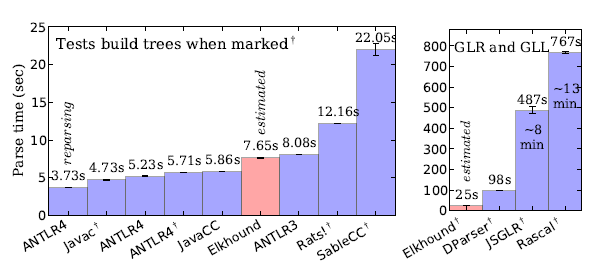
\includegraphics[scale=0.67]{Figure9.png}
\caption{
Porównanie Java czasu parsowania dla 10 narzędzi i 8 strategii na
bibliotece Java 6 i źródłach kompilatora (mniejsze wartości oznaczają szybciej).
12'920 plików, 3.6M linii, wielkość 123M.
Opis narzędzia zawiera: “tool name version [strategy].” ANTLR4 4.1 [ALL(*)]; Javac
7 [ręcznie zbudowany parser zejść rekurencyjnych i pierwszeństwa dla wyrażeń];
JavaCC 5.0 [LL(k)]; Elkhound 2005.08.22b [GLR] (testowany na Windows); ANTLR3 3.5 [LL(*)];
Rats! 2.3.1 [PEG]; SableCC 3.7
[LALR(1)]; DParser 1.2 [GLR]; JSGLR (z Spoofax) 1.1 [GLR];
Rascal 0.6.1 [GLL]. Testy uruchomione 10x z obfitą pamięcią, średnia/stddev
obliczona dla ostatnich 8 do uniknięcia kosztu JIT. Słupki błędów są znikome
ale pokazują pewne niestałości z powodu działania garbage collectora.
Aby uniknąć logarytmicznej skali, użyliśmy oddzielnego obrazka dla czasu parsowania GLR, GLL.
}
\end{figure}

\begin{figure}[h]
\begin{tabular}{|r||r|r|}
\hline
Tool & Time & RAM(M)\\
\hline\hline
$Javac^t$ & 89 ms & 7 \\
\hline
ANTLR4 & 201 ms & 8 \\
\hline
JavaCC & 206 ms & 7 \\
\hline
$ANTLR4^t$ & 360 ms  & 8 \\
\hline
ANTLR3 & 1048 ms &  143\\
\hline
$SableCC^t$ & 1'174 ms & 201 \\
\hline
$Rats!^t$ & 1'365 ms & 22 \\
\hline
$JSGLR^t$ & 15.4 sec & 1'030 \\
\hline
$Rascal^t$ & 24.9 sec & 2'622 \\
\hline
(no DFA) ANTLR4 & 42.5 sec & 27 \\
\hline
$elkhound^a$ & 3.35 min & 3 \\
\hline
$DParser^t$ & 10.5 hours & 100+ \\
\hline
$elkhound^t$ & out of mem & 5390+ \\
\hline
\end{tabular}
\caption{Czas i pamięć użyta do parsowania i opcjonalnego budowania drzew dla
3.2M pliku Java. Rozmiar pamięci jest medianą podawaną po GC podczas parsowania używając
-XX:+PrintGC opcji (dla C++ process monitoring). Czasy obejmują lexing; all input preloaded.
$^t$ Budowanie drzew; $^a$ Niejednoznaczność podczas parsowania, bez drzew}
\end{figure}

Nasz pierwszy eksperyment porównuje prędkość parsowania Java przez 10 narzędzi
i 8 strategii parsowania: ręcznie-wyregulowany zejść rekurencyjnych
z parsowaniem pierwszeństwa, LL(k), LL(*), PEG, LALR(1), ALL(*)
GLR, i GLL. Rysunek 9 pokazuje czas dla każdego narzędzia parsowania
12'920 plików źródłowych biblioteki Javy 6 i kompilatora.
Wybraliśmy Javę ponieważ miała ona najbardziej dostępną gramatykę wśród narzędzi
i przykładowe źródła Javy są obfite.
Gramatyki Java użyte w eksperymencie przyszły bezpośrednio z powiązanymi narzędziami
z wyjątkiem DParser i Elkhound, które nie oferowały odpowiedniej gramatyki Javy.
Przenieśliśmy gramatykę Java ANTLR do meta-składni tych narzędzi używając
jednoznacznych reguł wyrażeń arytmetycznych. Również osadzone akcje merge w
gramatyce Elkhound do ujednoznacznienia podczas parsowania do imitacji
rozdzielczości ANTLR w niejednoznaczności. Wszystkie pliki input były
ładowane do RAM przed parsowaniem i czasy odzwierciedlają średni czas obliczony
przez 10 całkowitych przejść korpusu, opuszczając dwa pierwsze dla
upewnienia się że nie mamy do czynienia z rozgrzewką kompilatora JIT.
Dla ALL(*) użyliśmy dwufazowego parsowania z Sekcji 3.2.
Testową maszyną był 6 core 3.33Ghz 16G RAM Mac OS X 10.7 desktop mający uruchomioną
Java 7 virtual machine. Elkhound and DParser parsers were
implemented in C/C++, które nie miały garbage collectora biegnącego równolegle.
Elkhound był ostatnio uaktualniony w 2005 roku
i dłużej nie był bufowany na Linuxie czy OS X, ale byliśmy w stanie zbudować go na
Windows 7 (4 core 2.67Ghz 24G RAM). Elkhound również mógł jedynie czytać z
pliku tak że Elkhound czas parsowania jest nieporównywalny.
W wysiłku by kontrolować prędkość maszyny różnice RAM kontra SSD, obliczyliśmy
współczynnik naszej Java test rig na naszej maszynie OS X czytającej z RAM do
ANTLR4
Javac
ANTLR4
ANTLR4
JavaCC
Elkhound
ANTLR3
Rats!
SableCC
5 0
10
15
20
25
Parse time (sec)
3.73s 4.73s 5.23s 5.71s 5.86s
7.65s 8.08s
12.16s
22.05s
estimated
reparsing
Tests build trees when marked
Elkhound
DParser
JSGLR
Rascal
0
100
200
300
400
500
600
700
800
25s
98s
487s
767s
GLR and GLL
estimated
~13
min
~8
min
test rig uruchomiony pod Windows z SSD. Nasze czasy Elkhound są w czasie Windows
pomnożonym przez współczynnik OS X do Windows.
\par
Dla tego eksperymentu, ALL(*) wyprzedza inne generatory parserów i jest
jedynie 20% wolniejszy niż parser zbudowany ręcznie w Javie. Kiedy porównywanie
uruchomione z konstrukcją drzewa (oznaczone przez † na Rysunku 9), ANTLR 4 jest
około 4.4x szybszy niż Elkhound, najszybsze narzędzie GLR które testowaliśmy,
i 135x szybsze niż GLL (Rascal). ANTLR 4 is niedeterministyczny ALL(*) parser
był nieco szybszy niż JavaCC’s deterministyczny LL(k) parser i około
2x szybszy niż Rats!’s PEG. W oddzielnym teście, wyszło że ten ALL(*)
wyprzedza Rats! Na jego własnej gramatyce PEG konwertowanej na składnięANTLR
(8.77s vs 12.16s).
Parser LALR(1) nie wykonywał dobrze przeciw narzędziom LL ale on mógłby
być SableCC’s implementacją a nie niedociągnięcie LALR(1). (Gramatyka Java z JavaCUP,
inny narzędzie LALR(1), było niekompletne i nie mogło parsować korpusu.)
Kiedy reparsowaliśmy korpus, ALL(*) lookahead z powodu trafień cache jest
szybsze 3.73s. Kiedy reparsowaliśmy z konstrukcją drzewa (czas nie pokazany),
ALL(*) pokonał ręcznie budowane Javac (4.4s kontra 4.73s).
Prędkość ponownego parsowania jest kwestią dla narzędzi takich jak środowisko deweloperskie.
\par
Parsery GLR które testowaliśmy są nawet o dwa rzędy wielkości wolniejsze w
parsowaniu Javy niż ALL(*). Z narzędzi GLR,
Elkhound ma najlepszą wydajność ponieważ polega on na liniowym stosie
LR(1) zamiast GSS gdzie możliwe.
Dalej, pozwoliliśmy Elkhound pozbyć się niejednoznaczności podczas
parsowania jak ALL(*). Elkhound używa oddzielnego lexera, w odróżnieniu od
JSGLR i DParser, które nie mają skanera.
Możliwe wyjaśnienie dla obserwowanej różnicy wydajności z ALL(*) jest
ze gramatykę Java przenieśliśmy do Elkhound i Dparser jest
stronniczy w kierunku ALL(*), ale ten zarzut nie jest zasadny.
GLR powinien także korzystać z wysoko deterministycznej i jednoznacznej gramatyki.
GLL było najwolniejsze w tym teście może dlatego że zespół Rascala przeniósł SDF GLR gramatykę Java,

a
Ujednoznacznienie poprzez parsowanie, bez drzew, szacowany czas.
Który jest nie optymalizowany dla GLL (wariacje gramatyki mają wpływ na wydajność.)
Rascal jest również bez skanera i jest obecnie jedynym dostępnym narzędziem GLL.
\par
Największym problemem z generalnymi algorytmami jest to że one są wysoko nieprzewidywalne
jeśli chodzi o czas i pamięć, które mogą czynić je nieodpowiednie dla
niektórych komercyjnych aplikacji. Obrazek 10 podsumowuje wydajność tych
samych narzędzi z pojedynczym plikiem Java 3.2M. Elkhound wzięte 7.65s do parsowania 123M Java
korpus, ale wzięte 3.35 minuty do parsowania pliku Java 3.2M. Spowodował on
błąd (out of memory) z konstrukcją lasu parsowania.
Czas DParsera skoczył z czasu korpusu 98s do 10.5 godzin.
na pliku 3.2M file. Prędkość Rascala JSGLR skalowały się miarę dobrze do 3.2M pliku,
ale użyły 2.6G and 1G RAM, odpowiednio.
W przeciwieństwie, ALL(*) parsował plik 3.2M w 360ms z konstrukcją drzewa używając 8M.
ANTLR 3 jest szybki ale jest wolniejszy i używa więcej pamięci (z powodu wstecznego pamiętania) niż ANTLR 4.
